\chapter{Simetrías y reglas de conservación}

\section{}

\section{}

\section{Grupo no-conmutativo: las rotaciones y el momentum angular}

Aplicar propiedades generales a problemas específicos, pero el grupo de rotaciones no es conmutativo.

Suponer un hamiltoniano $\hat{H}$ invariante ante rotaciones:

\begin{align*}
    \left[\hat{R}_{\vec{\mu}}(\alpha),\hat{H}\right]&=0\\ 
    \left[\hat{R}_{\vec{\mu}}(\alpha),\hat{U}(t)\right]&=0
\end{align*}

Tomamos una rotación de un ángulo $\alpha$ al rededor de $z$:

\begin{align*}
    \phi'(r,\theta,\phi)
        &=\hat{R}_z(\alpha)\phi(r,\theta,\phi)\\
        &=\phi(r,\theta,\phi+\alpha)
\end{align*}

Por definición de generador, el generador $\hat{L}_z$ es tal que $\hat{R}_z(\alpha)=\exp\left(-\frac{i}{\hbar}\hat{L}_z\alpha\right)$.

\subsection{Escritura vectorial}

\begin{align*}
    \hat{\vec{L}}=\hat{\vec{r}}\times\hat{\vec{p}}=
    \begin{cases}
        \hat{L}_x=\hat{y}\hat{P}_z-\hat{z}\hat{P}_y=-i\hbar(y\dd z-z\dd y)\\
        \hat{L}_y=\hat{z}\hat{P}_x-\hat{x}\hat{P}_z=-i\hbar(z\dd x-x\dd z)\\
        \hat{L}_z=\hat{x}\hat{P}_y-\hat{x}\hat{P}_y=-i\hbar(x\dd y-y\dd x)
    \end{cases}
\end{align*}

\subsection{Relaciones de conmutación}

Las relaciones de conmutación de $\hat{\vec{L}}$ están dadas por:

\begin{equation}
    \left[\hat{L}_i,\hat{L}_j\right]=i\hbar\varepsilon_{ijk}\hat{L}_k
\end{equation}

\subsection{Espacio de representaciones}

Un espacio invariante ante un grupo de transformaciones, se le llama espacio de representaciones del grupo.
Puede ser reducible si existe una suma directa de subespacios que sean invariantes ante este mismo grupo.

\subsubsection{Espacio de representaciones irreducibles de un grupo conmutativo}

\textbf{Propiedad:} Todas las representaciones irreducibles son de dimensión 1.

\subsubsection{Espacio de representaciones irreducibles de los grupos de rotación $SU(2)$ y  $SO(3)$}

Nos vamos a interesar en los generadores de rotaciones (operadores hermíticos y unitarios).

\textbf{Propiedad:}
Sean $\hat{J_x},\hat{J_y},\hat{J_z}$  operadores autoadjuntos en un espacio de Hilbert $\mathbb{H}$ que verifican el álgebra de Lie del grupo de rotaciones:

\begin{align}
    \left[J_i,J_j\right]=i\hbar\varepsilon_{ijk}\hat{J}_k
\end{align}

entonces ${\hat{\vec{J}}}^2$ conmuta con los elementos del álgebra de Lie.

\begin{align*}
    \left[{\hat{\vec{J}}}^2,\hat{J_i}\right]=0 \text{ para } i=x,y,z
\end{align*}

El espectro común de $J_z$ y $\vec{J}^2$ es de la forma:

\begin{align}
    \vec{J}^2\ket{j,m}&=\hbar^2j(j+1)\ket*{j,m}\\
    J_z\ket*{j,m}&=
\end{align}

Definimos los operadores escalón:

\begin{align*}
    J_+&=J_x+iJ_y\\
    J_-&=J_x-iJ_y
\end{align*}

Y notamos que $J_+^\dagger=J_-$

Las relaciones de conmutación:

\begin{align*}
    \left[J_+,J_-\right]&=2\hbar J_z\\
    \left[J_z,J_\pm\right]&=\pm \hbar J_{pm}\\
    \left[\vec{J}^2,J_{\pm}\right]&=0
\end{align*}

\medskip


Con $j$ fijo, los vectores $\ket*{j,m}$, con $m=-j,\cdots,j$ forman una base ortonormal $(\bra*{j,m}\ket*{j,n}=\delta_{mn})$ de un espacio vectorial $D_j$ de dimensión $j+1$ y el espacio $D_j$ es un espacio de representaciones irreducibles del grupo de rotación.

Todo espacio de representaciones del grupo de rotaciones puede descomponerse como la suma de espacios irreducibles $$H=D_{j1} \oplus D_{j2} \oplus\cdots$$ (con índices que pueden repetirse).

\bigskip

\hspace{1cm}\textbf{Nota:} Los 3 generadores $J_x,J_y,J_z$ forman una base del álgebra de Lie llamada álgebra de Lie $SO(3)$ o $SU(2)$. Los generadores $J_x,J_y,J_z$ forman otra base de la misma álgebra más interesante. A esta base se le llama descomposición de Cartan de $SU(2)$, $SO(3)$ complejificada.

Tenemos que:

\begin{align*}
    J_z\left(J_\pm \ket*{a,m}\right)
        &=\left(\left[J_z,J_\pm\right]+J_\pm J_z\right)\ket*{a,m}\\
        &=\pm \hbar J_\pm \ket*{a,m}+\hbar mJ_\pm\ket*{a,m}\\
        &=\hbar(\pm1+m)J_\pm\ket*{a,m}
\end{align*}

por otro lado,

\begin{align*}
    \vec{J}^2\left(J_\pm\ket*{a,m}\right)=J_\pm \vec{J}^2 \ket*{a,m}=\hbar^2aJ_\pm\ket*{a,m}
\end{align*}

\textbf{Nota:}

\begin{align*}
    \vec{J}^2=\frac{1}{2}\left(J_+J_-+J_-J_+\right)J_z^2
\end{align*}

Entonces notemos que:

\begin{align*}
    \hbar^2(a-m^2)
        &=\bra{a,m}\vec{J}^2-J_z^2\ket{a,m}\\
        &=-\frac{1}{2}\bra{a,m}\left(J_+J_-+J_-J_+\right)\ket{a,m}\\
        &\geq 0\\
    a&\geq m^2
\end{align*}

Existe un valor máximo de $m:m_{max}$, y por tanto un mínimo. 

Esto se traduce en:

\begin{align*}
    J_+\ket{a,m_{max}}&=0\\
    J_-\ket{a,m_{min}}&=0
\end{align*}

Por otro lado,

\begin{align*}
    \vec{J^2}
        &=J_z^2+\frac{1}{2}\left(J_+J_-+J_-J_+\right)\\
        &=J_z^2+J_+J_--\hbar J_z
\end{align*}

Aplicamos la relación a $\ket{a,m_{max}}$ y a $\ket{a,m_{min}}$:

\begin{align*}
    \vec{J}^2\ket{a,m_{max}}
        &=\hbar^2a^2\ket{a,m_{max}}\\
        &=\\
        &=\hbar^2 m_{max} (m_{max}+1)\ket{a,m_{max}}
\end{align*}

$$a^2=m_{max}(m_{max}+1)$$

de igual manera $a^2=m_{min}(m_min-1)$.

\medskip

Dado que $J_z\left(J_{\pm}\ket{a,m}\right)=\hbar(\pm1+m)(J_\pm\ket{a,m})$ podemos definir:

\begin{align}
    \ket{a,m=m\pm1}=\frac{1}{c_\pm}J_\pm\ket{a,m}
\end{align}

podemos intuir que $m_{max}=m_{min}+n$ con $n\in \mathbb{N}$ entonces:

\begin{align}
    a^2=m^2_{max}+m_{max}=m_{min}^2+m_{min}
\end{align}

De esto: $m_{min}=-\frac{n}{2}$ y por tanto $m_{max}=m_{min}+n=\frac{n}{2}=j$.

Por tanto $m=-j,-j+1,\cdots,j-1,j$ y tenemos $(2j+1)$ valores posibles.

Ahora la normalización $c_\pm$, si $\ket{j,m}$ está normalizado,

\begin{align*}
    \abs{c_{\pm}}^2\norm*{\ket{j,m+1}}^2
        &=\bra{j,m}J_-J_+\ket{j,m}\\
        &=\hbar^2 \left(j(j+1)-m(m+1)\right)
\end{align*}

de igual manera para $c_-$.

Por tanto, cada espacio $D_j$ es de dimensión $(2j+1)$ y los operadores $J_\pm$, $J_z$ actúan dentro de $D_j$ al igual que $J_x,J_y,J_z$ que se obtienen por medio de combinaciones lineales. 

$D_j$ es invariante ante rotaciones: es un espacio de representación del grupo de rotación.

Cada $D_j$ no puede descomponerse en la suma de 2 espacios. 

\hfill$\qed$

\subsection{En resumen: Representaciones irreducibles de los grupos de rotación $SO(3)$ y $SU(2)$}

Recordemos que:

\begin{align*}
    \vec{J}^2\ket{j,m}=\hbar^2j(j+1)\ket{j,m}\\
    J_z\ket{j,m}=\hbar m\ket{j,m}
\end{align*}

Vamos a tomar ahora al estado $\ket{j,m}$ y lo vamos a rotar por $2\pi$ al rededor de $z$.

\begin{align*}
    R_z(2\pi)
        &=\pm\ket{j,m}
\end{align*}

$+$ si $m$ es entero, y $-$ si $m$ es medio entero.

Entonces:

Si $D_j$ es una representación de $SO(3)$, entonces $R(2\pi)=\mathbb{I}$ $\Rightarrow j$ (y por tanto $m$ también) debe ser un entero.

$$
\rightarrow l=j=0,1,2,\cdots
$$

así, el espacio de representaciones irreducibles de $SO(3)$ son los espacios $D_l$ caracterizados por el entero $l$. Notemos que $D_l$ es de dimensión impar $(2l+1)$.

Si $D_j$ es una representación de $SU(2)$ (rotación de espín $1/2$) $\Rightarrow R(4\pi)=\mathbb{I}$, entonces los valores de $j$ permitidos son:

$$
j=0,1/2,1,\cdots
$$

Los espacios de representación irreducibles de $SU(2)$ son los espacios $D_j$ caracterizados por el entero o medio entero $j$.

\textbf{Nota:}
\begin{itemize}
    \item Del hecho que $\left[\vec{J}^2,\vec{J}\right]=0\Rightarrow\left[J^2,R\right]=0$ para cualquier operador de rotación.
    $$
    R_\mu (\theta)=\exp()
    $$
    Decimos que $\vec{J}^2$ es un operador de Casimir del grupo de rotación.
    Uno de los espacios de representación irreducibles $D_j$ es el espacio propio de $\vec{J}^2$ caracterizado por el autovalor $\hbar^2 $

    \item Los vectores $\ket{j,m}$ forman una base de $D_j$. Estos vectores son autovectores de $J_z$ y la dirección de esta base depende de la elección del eje $z$
\end{itemize}

\textbf{Ejemplos}

\begin{enumerate}
    \item Para describir el espín $1/2$, el espacio $\mathbb{H}_{espin}=\mathbb{C}^2$ de dimensión 2 y los operadores $S_x,S_y,S_z$ y se identifican con el espacio $D_{1/2}$ para $j=1/2$.
    \item El espacio $\mathbb{R}^3$ es un espacio de representaciones irreducible de $SO(3)$. $\mathbb{R}^3$ se identifica al espacio $D_{l=1}$ con base $\ket{l=1,m=-1,0,+1}$ que identificamos con $\ket{x},\ket{y},\ket{z}$ de la siguiente manera:
    \begin{enumerate}
        \item vamos a escribir
    \end{enumerate}
\end{enumerate}


\subsubsection{Aplicación: espectro de un rotor rígido:}

Tomar el ejemplo de una molécula diatómica $(HCl,NaCl,H_2,O_2,\cdots)$, vamos a ignorar la vibración de la molécula y la traslación $\Rightarrow$ solo consideramos rotaciones en ella misma:

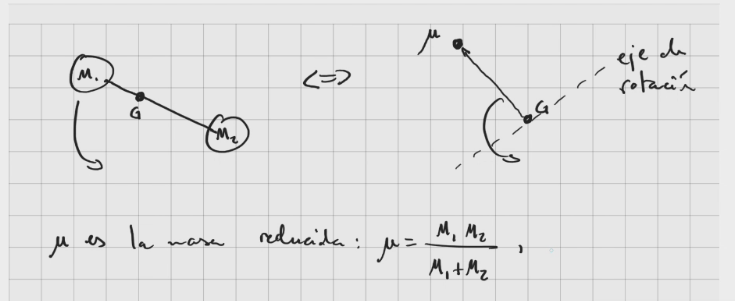
\includegraphics[width=0.4\textwidth]{Graficas/G1-Aug2.png}

\textbf{El espacio de Hilbert de los estados cuánticos:}

Movimiento reducido a una esfera $S^2$

$$
\mathbb{H}=L^2(S^2)
$$

los vectores son funciones de onda $\Psi(\theta,\phi)$ en un punto $(\theta,\phi)$ sobre la esfera.
La esfera es el espacio de configuraciones del sistema.

Denotamos por $\ket{\theta,\phi}$ al estado de la posición (delta de Dirac en el punto).

$$
\psi(\theta,\phi)=\bra{\theta,\phi}\ket{\psi}
$$

y la resolución de la identidad:

Donde $\dd\Omega$ es el ángulo sólido de la esfera.

\textbf{Operador Hamiltoniano:}

En el caso clásico:

\begin{align*}
    H=\frac{1}{2}\mu v^2=\frac{1}{2} \mu r_o^2\omega^2=\frac{L^2}{2I}
\end{align*}

con $I$ el momento de inercia $I=\mu r_o^2$ y $L$ el momentum angular.

Cuantizamos 
$$
\hat{H}=\frac{\hat{I}^2}{2I}
$$

con $\vec{L}^2=L_x^2+L_y^2+L_z^2$

\textbf{Espectro de $\hat{H}$}

Teorema: En el espacio de hilbert $\mathbb{H}=L^2(S^2)$, cada espacio de representaciones irreducibles $D_l$, $l=0,1,2,\cdots$ aparece solo una vez:

\begin{align*}
    \mathbb{H}=L^2(s^2)=\bigoplus_{l=0}^\infty D_l
\end{align*}


\subsection{Importancia de las representaciones irreducibles:}

\subsubsection{Propiedades fundamentales: el lema de Schur y el teorema de Wigner}

El lema de Schur tiene varias formulaciones, pero la más útil en mecánica cuántica es la siguiente:

\textbf{Lema de Schur:} Sea $\hat{A}:\mathbb{H}\rightarrow\mathbb{H}$ un operador que actúa sobre el espacio de Hilbert $\mathbb{H}$. Vamos a suponer que este es la suma directa de espacios irreducibles de un grupo $G$, que pos simplicidad diremos que son $2$.

\begin{equation*}
    \mathbb{H}=D_j\oplus D_k\tag{1}
\end{equation*}

y estas representaciones no son equivalentes:
$$
D_j\neq D_k
$$
Bien $j\neq k$ y además para todo $\hat{G}\in G$
$$
\left[A,G\right]=0
$$
$g$ es un grupo de simetrías de $\hat{A}$. Entonces $\hat{A}$ se escribe respecto a la descomposición $(1)$ como:

$$
\hat{A}=\begin{pmatrix}
    a_j\mathbb{I} & 0\\
    0 & a_k\mathbb{I}
\end{pmatrix}
$$

(el resultado es generalizable a la suma de más representaciones irreducibles)

\textbf{Prueba:} Para esto necesitaremos 2 lemas intermedios:

\textbf{Lema de Schur A:} Si $\hat{A}:D_j\rightarrow D_k$ es un operador lineal entre 2 espacios de representaciones irreducibles de $G$ y $\left[A,G\right]=0$ $\forall \hat{G}\in G$ entonces $A=0$ o bien $A$ es un isomorfismo $\Rightarrow D_j\approxeq D_k,j=k$

Nota: 
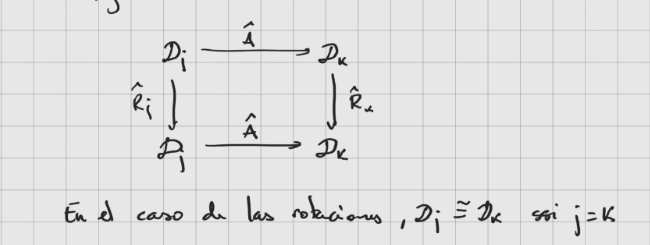
\includegraphics[width=0.4\textwidth]{Graficas/G2-Aug2.png}

\textbf{Prueba:} El Kernel de $A$, $\ker A\subset D_j$ es invariante por $G$. En efecto, si $\psi\in\ker A$, i.e. $A\psi=0$ entonces sean $\psi '=G\psi$ entonces:

\begin{align*}
    A\psi ' =AG\psi=GA\psi=0\Rightarrow\psi ' \in\ker A
\end{align*}

Ahora bien, $D_j$ es irreducible $\Rightarrow \ker A=\{0\}\Rightarrow A$ es inyectiva o $A=0$.

Por otro lado, $Im(A)\subset D_k$ es invariante por $G$. En efecto, si $\psi \in Im(A)$, $\psi=A\phi\Rightarrow\psi'\in Im(A)$ Como $D_k$ es irreducible, $Im(A)=0$ o $Im(A)=D_k$ (es sobreyectiva).

Por tanto, $A=0$ o $A$ es isomorfismo.

\textbf{Lema de Schur B:}

Si $A:D_j\rightarrow D_k$ es un operador lineal en un espacio de representaciones irreducibles de $G$ y $\left[A,G\right]=0 \forall \hat{G}\in G$ entonces $A=a\mathbb{I}$ con $a\in \mathbb{C}$

\textbf{Prueba:}
Los espacios propios de $A$ denotados $\mathbb{H}_a\subset D_j$ son invariantes por la acción de $G$. Pero $D_j$ es irreducible. Entonces solo hay uno.

El resto de la prueba se basa en escribir al operador $A$ como una matriz de $2\times 2$ utilizando proyecciones, donde los elementos de matriz $A_{ab}$ están dados por $P_a A p_b$. Y por tanto:

\begin{align*}
    \begin{pmatrix}
        a_j \mathbb{I} & 0\\
        0 & a_k \mathbb{I}
    \end{pmatrix}
\end{align*}


\textbf{Teorema de Wigner}
Si el hamiltoniano $\hat{H}$ tiene un espectro discreto y admite una simetría por un grupo de invarianza G discreto o continuo, i.e.$$\left[H,G\right]=0\forall G\in G$$

entonces genéricamente (el resultado de toda perturbación respecto a esta simetría es estable), los espacios propios de $H$ son representaciones irreducibles de $G$.

En particular, si el grupo $G$ es conmutativo, sus representaciones irreducibles son de dimensión $1$ y esperaríaos que no haya degeneración en el espectro, i.e. todos los niveles son distintos (momentum de espectro continuo),
Si el grupo es no conmutativo, entonces admite representaciones irreducibles de dimensión $d\geq 1$ y esperamos degeneraciones en el espectro de multiplicidad $d$. (i.e. distintos estados con misma energía).

\textbf{Nota:}
Esta propiedad resulta muy útil en física molecular: conociendo las representaciones irreducibles de distintos grupos (hay al menos 230 grupos finitos del espacio catalogados y observados en la naturaleza) y observando el espectro de una molécula, deducimos el grupo de invarianza y así podemos deducir la forma de la molécula (geométrica).

Espectro $\Rightarrow $ grupo de simetría $\Rightarrow$ forma de la molécula.

\textbf{Ejemplo: El espectro del átomo de hidrógeno}

\textit{Repaso:}

\begin{align*}
    \hat{H}=\frac{\hat{\vec{p}}^2}{2m}-\frac{e^2}{4\pi\epsilon_o}\frac{1}{r} 
\end{align*}

por el momento no tomamos en cuenta el espín. $\hat{H}$ es invariante ante rotaciones: $\left[\hat{H},\hat{T}\right]=0$. El espectro es tal que:

\begin{align*}
    \hat{H}\ket{\psi_{n,l,m}}=E_n\ket{\psi_{n,l,m}}   
\end{align*}


los autovectores son el producto de una función radial y de armónicos esféricos:

\begin{align*}
    \bra{x}\ket{\psi_{n,l,m}}=R_{n,l}(r)Y_{l,m}(\theta,\psi)
\end{align*}

Con $E_n=$

Cada uno de los niveles de energía constituye entonces un espacio propio 

\begin{align*}
    H_n=\bigoplus_{l=0}^{n-1}D_l
\end{align*}

Este espacio es de dimensión $n^2$

$$
\left(\sum_{l=0}^{n-1}(2l+1)=n^2\right)
$$

\textbf{Simetría adicional de Pauli, y degeneración a $l$:}

Esto pareciera contradecir el teorema de Wigner

De hecho no lo contradice, ya que el potencial tiene una forma muy particular, está en términos de $1/r$ y esto hace que haya una simetría más (descubierta por Pauli en $1925$), cuyo generador es:

\begin{align*}
    \hat{\vec{A}}=\frac{1}{2m}\left(\vec{p}\times\vec{L}-\vec{L}\times\vec{p}\right)-mK\frac{\vec{x}}{\abs{x}}
\end{align*}

con $K=\frac{e^2}{4\pi\epsilon}$ y $\vec{A}$ se conoce como el vector de Runge Lenz.

Es posible verificar que:

\begin{align*}
    \left[A,H\right]=0
\end{align*}

El grupo de simetrías es ahora $SO(4)$ de dimensión $6$ y cada espacio propio $H$ es irreducible para esta simetría.

Podemos romper esta simetría: correcciones relativistas. (rompen la simetría de $A$ pero no la invarianza rotacional)



